\documentclass[10pt,a4paper]{article}
\usepackage[utf8]{inputenc}
\usepackage[german]{babel}
\usepackage{mathrsfs}
\usepackage{amsmath}
\usepackage{amsfonts}
\usepackage{amssymb}
\usepackage{amsthm}
\usepackage[left=2cm,right=2cm,top=2cm,bottom=2cm]{geometry}
\usepackage{listings}
\usepackage{graphicx}

\begin{document}

\section{Aufgabe 17}

\subsection{$\mathbb{P}_{0}$}

Gesucht ist das Polynom $g(x) = \alpha_{0} \in \mathbb{P}_{0}$.
\begin{equation}
  (1, 1)\alpha = \alpha = (\sqrt{x}, 1) = \int_{0}^{1} \sqrt{x} dx = [\frac{2}{3}x^{\frac{3}{2}}]_{0}^{1} = \frac{2}{3}
\end{equation}
\begin{equation}
  g(x) = \frac{2}{3}
\end{equation}

\begin{lstlisting}
x = 0:0.01:1;

figure;
hold on;
plot(x, sqrt(x), 'c', 'LineWidth', 3, 'DisplayName', 'sqrt(x)');
plot(x, ones(1, length(x)) * 2/3, 'r', 'LineWidth', 3, 'DisplayName', 'g(x)');
hold off;
legend('show');
\end{lstlisting}

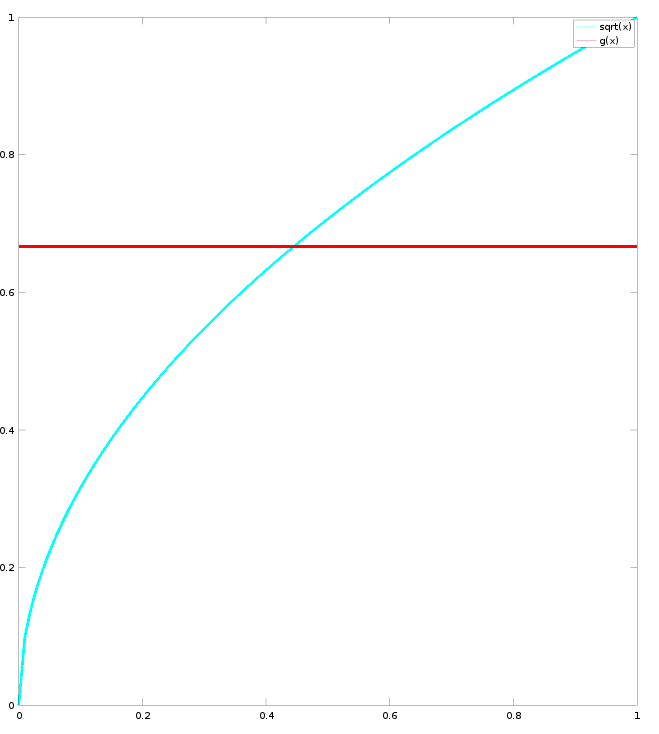
\includegraphics[width=300pt]{6_17_p0.png}

\subsection{$\mathbb{P}_{1}$}

Gesucht ist das Polynom $g(x) = \alpha_{1}x + \alpha_{0} \in \mathbb{P}_{1}$.
\begin{align*}
  \begin{pmatrix}
    (1, 1) & (1, x)\\
    (x, 1) & (x, x)
  \end{pmatrix}
  \cdot
  \begin{pmatrix}
    \alpha_{0}\\\alpha_{1}
  \end{pmatrix}
  & =
  \begin{pmatrix}
    (\sqrt{x}, 1)\\
    (\sqrt{x}, x)
  \end{pmatrix}
  \\
  \Leftrightarrow
  \begin{pmatrix}
    1 & \frac{1}{2}\\
    \frac{1}{2} & \frac{1}{3}
  \end{pmatrix}
  \cdot
  \begin{pmatrix}
    \alpha_{0}\\\alpha_{1}
  \end{pmatrix}
  & =
  \begin{pmatrix}
    \frac{2}{3}\\
    \frac{2}{5}
  \end{pmatrix}
  \\
  \Leftrightarrow
  \begin{pmatrix}
    \alpha_{0}\\\alpha_{1}
  \end{pmatrix}
  & =
  \begin{pmatrix}
    \frac{4}{15}\\
    \frac{4}{5}
  \end{pmatrix}
\end{align*}
\begin{equation}
  g(x) = \frac{4}{5}x + \frac{4}{15}
\end{equation}

\begin{lstlisting}
x = 0:0.01:1;

figure;
hold on;
plot(x, sqrt(x), 'c', 'LineWidth', 3, 'DisplayName', 'sqrt(x)');
plot(x, (4/5) * x + 4/15, 'r', 'LineWidth', 3, 'DisplayName', 'g(x)');
hold off;
legend('show');
\end{lstlisting}

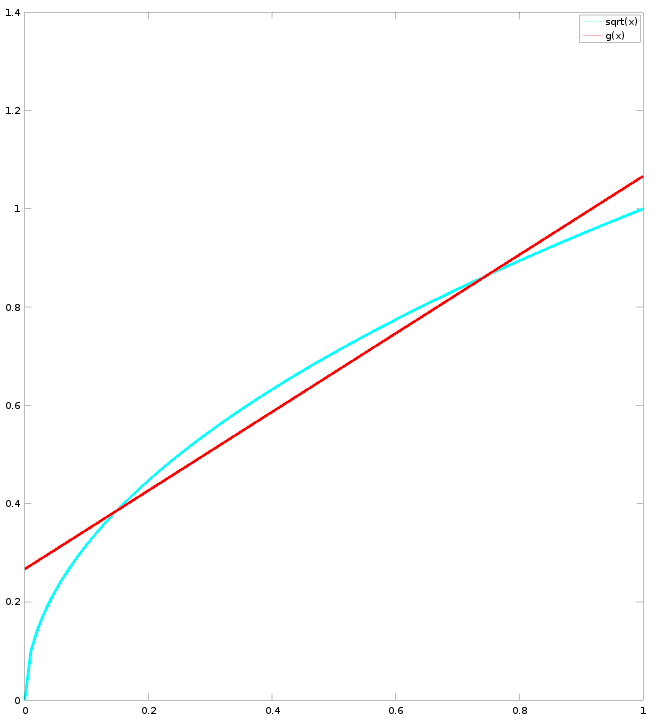
\includegraphics[width=300pt]{6_17_p1.png}

\subsection{$\mathbb{P}_{2}$}

Gesucht ist das Polynom $g(x) = \alpha_{2}x^{2} + \alpha_{1}x + \alpha_{0} \in \mathbb{P}_{2}$.
\begin{align*}
  \begin{pmatrix}
    (1, 1) & (1, x) & (1, x^{2})\\
    (x, 1) & (x, x) & (x, x^{2})\\
    (x^{2}, 1) & (x^{2}, x) & (x^{2}, x^{2})
  \end{pmatrix}
  \cdot
  \begin{pmatrix}
    \alpha_{0}\\\alpha_{1}\\\alpha_{2}
  \end{pmatrix}
  & =
  \begin{pmatrix}
    (\sqrt{x}, 1)\\
    (\sqrt{x}, x)\\
    (\sqrt{x}, x^{2})
  \end{pmatrix}
  \\
  \Leftrightarrow
  \begin{pmatrix}
    1 & \frac{1}{2} & \frac{1}{3}\\
    \frac{1}{2} & \frac{1}{3} & \frac{1}{4}\\
    \frac{1}{3} & \frac{1}{4} & \frac{1}{5}
  \end{pmatrix}
  \cdot
  \begin{pmatrix}
    \alpha_{0}\\\alpha_{1}\\\alpha_{2}
  \end{pmatrix}
  & =
  \begin{pmatrix}
    \frac{2}{3}\\
    \frac{2}{5}\\
    \frac{2}{7}
  \end{pmatrix}
  \\
  \Leftrightarrow
  \begin{pmatrix}
    \alpha_{0}\\\alpha_{1}\\\alpha_{2}
  \end{pmatrix}
  & =
  \begin{pmatrix}
    \frac{6}{35}\\
    \frac{48}{35}\\
    -\frac{4}{7}
  \end{pmatrix}
\end{align*}
\begin{equation}
  g(x) = -\frac{4}{7}x^{2} + \frac{48}{35}x + \frac{6}{35}
\end{equation}

\begin{lstlisting}
x = 0:0.01:1;

figure;
hold on;
plot(x, sqrt(x), 'c', 'LineWidth', 3, 'DisplayName', 'sqrt(x)');
plot(x, (-4/7) * (x.^2) + (48/35) * x + 6/35, 'r', 'LineWidth', 3, 'DisplayName', 'g(x)');
hold off;
legend('show');
\end{lstlisting}

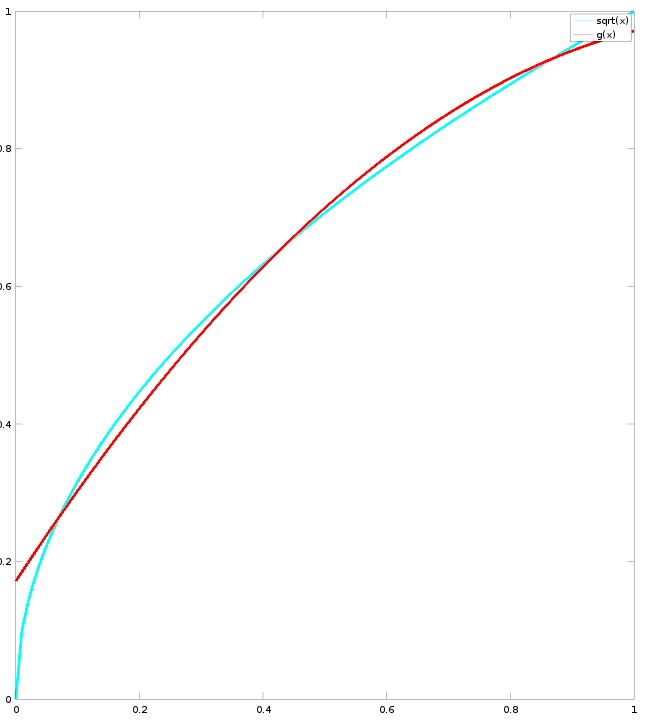
\includegraphics[width=300pt]{6_17_p2.png}

\section{Aufgabe 18}

\section{Aufgabe 19}

\subsection{Teil 1}

Berechnung mit dem Gram-Schmidt-Algorithmus
\begin{equation}
  \varphi_{1} = 1
\end{equation}
\begin{equation}
  \tilde{\varphi}_{2} = x - (x, 1) = x - \frac{1}{2}
\end{equation}
\begin{equation}
  \varphi_{2} = \frac{\tilde{\varphi}_{2}}{||\tilde{\varphi}_{2}||} = \frac{x - \frac{1}{2}}{\sqrt{(x - \frac{1}{2}, x - \frac{1}{2})}} = \frac{x - \frac{1}{2}}{\sqrt{\frac{1}{12}}} = \sqrt{12}(x - \frac{1}{2})
\end{equation}
\begin{equation}
  \tilde{\varphi}_{3} = x^{2} - (1, x^{2}) - (\sqrt{12}(x - \frac{1}{2}), x^{2}) \cdot \sqrt{12}(x - \frac{1}{2}) = x^{2} - \frac{1}{3} - x + \frac{1}{2} = x^{2} - x + \frac{1}{6}
\end{equation}
\begin{align*}
  \varphi_{3} & = \frac{\tilde{\varphi}_{3}}{||\tilde{\varphi}_{3}||}\\
  & = \frac{x^{2} - x + \frac{1}{6}}{\sqrt{(x^{2} - x + \frac{1}{6}, x^{2} - x + \frac{1}{6})}}\\
  & = \frac{x^{2} - x + \frac{1}{6}}{\sqrt{\frac{1}{180}}}\\
  & = \frac{x^{2} - x + \frac{1}{6}}{\frac{1}{6 \sqrt{5}}}\\
  & = (6 \sqrt{5})(x^{2} - x + \frac{1}{6})
\end{align*}

\begin{equation}
  (1, \sqrt{12}(x - \frac{1}{2}), (6 \sqrt{5})(x^{2} - x + \frac{1}{6}))
\end{equation}
ist also eine Orthonormalbasis von $\mathbb{P}_{2}$.

\subsection{Teil 2}

Da wir eine Orthonormalbasis haben, können wir die Koeffizienten der Bestapproximation $g = \alpha_{1} \varphi_{1} + \alpha_{2} \varphi_{2} + \alpha_{3} \varphi_{3}$ direkt bestimmen.
\begin{equation}
  \alpha_{1} = (f, \varphi_{1}) = \int_{0}^{1} f(x) dx = [\frac{2}{3}x^{\frac{3}{2}}]_{0}^{1} = \frac{2}{3}
\end{equation}
\begin{equation}
  \alpha_{2} = (f, \varphi_{2}) = \int_{0}^{1} \sqrt{x}\sqrt{12}(x - \frac{1}{2}) dx = \sqrt{12} \int_{0}^{1} x \sqrt{x} - \frac{1}{2} \sqrt{x} dx = \sqrt{12} [\frac{2}{5}x^{\frac{5}{2}} - \frac{1}{3}x^{\frac{3}{2}}]_{0}^{1} = \frac{\sqrt{12}}{15}
\end{equation}
\begin{align*}
  \alpha_{3} & = (f, \varphi_{3}) = \int_{0}^{1} \sqrt{x}(6 \sqrt{5})(x^{2} - x + \frac{1}{6}) dx\\
  & = 6 \sqrt{5} \int_{0}^{1} x^{\frac{5}{2}} - x^{\frac{3}{2}} + \frac{1}{6} \sqrt{x} dx\\
  & = 6 \sqrt{5} [\frac{2}{7}x^{\frac{7}{2}} - \frac{2}{5} x^{\frac{5}{2}} + \frac{1}{9} x^{\frac{3}{2}}]_{0}^{1}\\
  & = 6 \sqrt{5} (\frac{2}{7} - \frac{2}{5} + \frac{1}{9}) = -6 \sqrt{5} \frac{1}{315} = -\frac{2 \sqrt{5}}{105}
\end{align*}
\begin{align*}
  g(x) & = \frac{2}{3} + \frac{\sqrt{12}}{15} \sqrt{12}(x - \frac{1}{2}) - \frac{2 \sqrt{5}}{105}(6 \sqrt{5})(x^{2} - x + \frac{1}{6})\\
  & = \frac{2}{3} + \frac{4}{5}(x - \frac{1}{2}) - \frac{12}{21}(x^{2} - x + \frac{1}{6})\\
  & = \frac{2}{3} + \frac{4}{5}x - \frac{2}{5} - \frac{12}{21}x^{2} + \frac{12}{21}x - \frac{2}{21}\\
  & = -\frac{4}{7}x^{2} + \frac{48}{35}x + \frac{6}{35}
\end{align*}

\section{Aufgabe 20}

\end{document}